% TEMPLATE for Usenix papers, specifically to meet requirements of
%  USENIX '05
% originally a template for producing IEEE-format articles using LaTeX.
%   written by Matthew Ward, CS Department, Worcester Polytechnic Institute.
% adapted by David Beazley for his excellent SWIG paper in Proceedings,
%   Tcl 96
% turned into a smartass generic template by De Clarke, with thanks to
%   both the above pioneers
% use at your own risk.  Complaints to /dev/null.
% make it two column with no page numbering, default is 10 point

% Munged by Fred Douglis <douglis@research.att.com> 10/97 to separate
% the .sty file from the LaTeX source template, so that people can
% more easily include the .sty file into an existing document.  Also
% changed to more closely follow the style guidelines as represented
% by the Word sample file.

% Note that since 2010, USENIX does not require endnotes. If you want
% foot of page notes, don't include the endnotes package in the
% usepackage command, below.

% This version uses the latex2e styles, not the very ancient 2.09 stuff.
\documentclass[letterpaper,twocolumn,10pt]{article}
\usepackage{usenix,epsfig,endnotes}
\usepackage{balance}
\usepackage{xcolor}
\usepackage{xspace}
\usepackage{program}
\usepackage[hyperfootnotes=false]{hyperref}

\hypersetup{
  citebordercolor=red
}

\begin{document}

%don't want date printed
\date{}

%make title bold and 14 pt font (Latex default is non-bold, 16 pt)
\title{\Large \bf CS598PS Report: Kaggle Accelerometer Biometric Competition}

%for single author (just remove % characters)
\author{
{\rm Hilfi Alkaff}\\
alkaff2@illinois.edu
\and
{\rm Efe Karakus}\\
karakus1@illinois.edu
\and
} % end author

\maketitle

% Use the following at camera-ready time to suppress page numbers.
% Comment it out when you first submit the paper for review.
\thispagestyle{empty}

\section{Problem}

For our CS598PS project, we entered a Kaggle competition that requires us to
identify mobile devices from accelerometer data~\cite{Kaggle2013}. Since
everyone moves differently and that most devices are being equipped with
accelerometers nowadays, the purpose of this competition is to investigate the
feasibility of deanonymizing users of mobile device from their accelerometer
data using machine learning techniques.

In the competition, approximately 60 million unique samples of accelerometer
data are collected from 387 different devices. These are split into equal sets
for training and test. Samples in the training set are labeled with the unique
device from which the data was collected. The test set is demarcated into 90k
sequences of consecutive samples from one device.

\begin{figure}
  \centering
  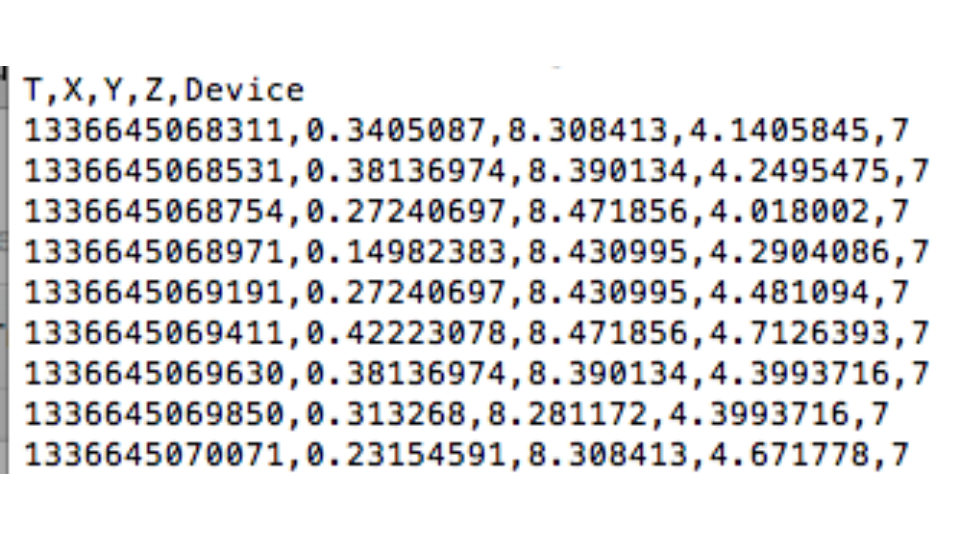
\includegraphics[width=\linewidth]{./figs/train_data.png}
  \caption{Format of training data.}
  \label{fig:train}
\end{figure}

\begin{figure}
  \centering
  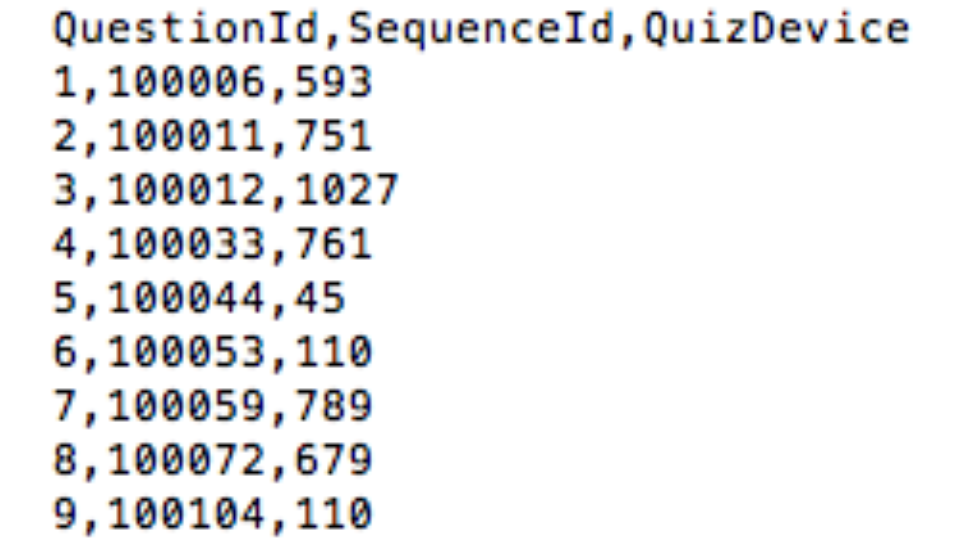
\includegraphics[width=\linewidth]{./figs/questions.png}
  \caption{Format of question data.}
  \label{fig:question}
\end{figure}

We are given two datasets mainly. The first dataset is the training data as
indicated in Figure~\ref{fig:train}. In this file, the format is that the first
field contains the timestamp, T, in which the data is being taken while the
next three fields indicate the coordinates of the accelerometer; X, Y, Z. The
last field contains the DeviceId which indicates the unique id of the device
that generated this particular data point. The second dataset is the question
data as indicated in Figure~\ref{fig:question}. In this file, the first field
is the id of the question, QuestionId, the second field is unique number
assigned to each sequence of sample, SequenceId, and the third field is the
professed device id that generated the sequence of accelerometer data that we
need to either agree or disagree to.

\section{Solution}

\subsection{Classification}
In this competition, since the data is organized in a time-series format

\subsection{Clustering}
In the previous section, we knew which device id we needed the test sequence
to compare to. If this information was not available to us, we would need
to do a linear scan through every device in the training set for every
test sequence. Hence, the runtime is \textit{O}($nm$) where $n$ is the
number of device ids and $m$ the number of test sequences. With our 
training and test data files, it took us ~15 hours to do classification.

An interesting sub-problem would be to find a cheap and efficient way of
doing search space reduction. We decided to apply the k-means clustering
algorithm~\cite{kmeans} to create $\sqrt{387} \simeq 20$ clusters, and only build HMMs
after finding which cluster the sequence is most likely part of. We used both
euclidian distance and cosine similarity as our distance measures between
clusters.

\begin{program}
\mbox{\textit{\textbf{k-means(devices, k)}}}
\BEGIN \\
  samples := randomsample(devices, k) \\
  clusters := [] \\
  \FOR sample <- samples \DO
    clusters.add([sample]) \OD
  means := findmeans(clusters) 
  \WHILE is\ not\ converged(clusters) \DO
    clusters := [[]\ for\ k]
    \FOR device <- devices \DO
      \FOR i <- 0..k \DO
        m = means[i]
        d = distance(device, m)
        \IF is\ best\ distance(d)
          clusters[i].add(device)
        \OD
        \OD
    means = findmeans(clusters)
    \OD
\END
\end{program}

The distance() function can be implemented with euclidian distance. In this
situation, we observe that the sizes of our clusters are very skewed.

\begin{figure}[h]
  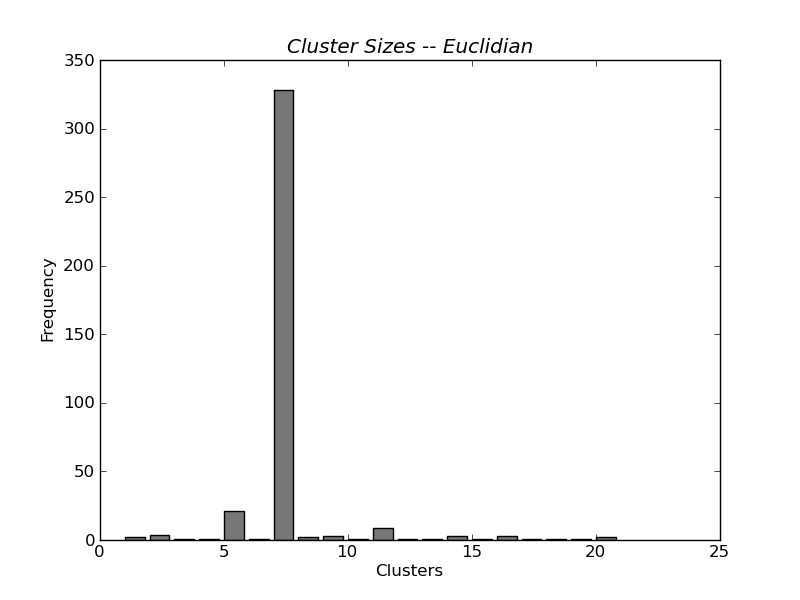
\includegraphics[width=\linewidth]{./figs/euclidian.png}
  \label{fig:euclidian}
\end{figure}

However, if we use cosine similarity as a distance measurements we get even
cluster sizes. Therefore, it is preferable to use cosine similarity as
the distance measurement.

\begin{figure}[h]
  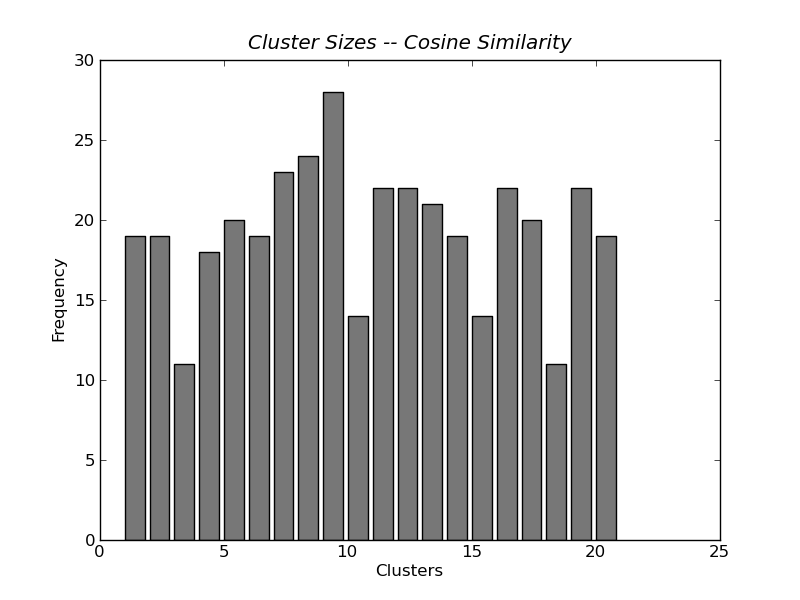
\includegraphics[width=\linewidth]{./figs/cosine.png}
  \label{fig:cosine}
\end{figure}


\section{Code}

Our code is open-sourced at \url{https://github.com/efekarakus/accelerometer-biometric-competition}.


\bibliographystyle{abbrv}
\bibliography{main}

\end{document}
